\subsection{Overall performance}

We evaluated several large language models (LLMs) on MeBench to assess their ability to identify TF-to-gene regulatory mechanisms and apply them in forward and inverse reasoning tasks. Our evaluation included five closed-book general-purpose models and the tool-augmented biomedical agent Biomni. Table~\ref{tab:model_performance} shows the evaluation results across three tasks using Task 1 balanced accuracy and macro-F1, and Task 2/3 balanced joint accuracy and protocol-specific joint F1. Task 1 balanced accuracy ranges from 26.9\% to 34.7\%, and macro-F1 ranges from 22.7\% to 34.5\% (Table~\ref{tab:model_performance}). GPT-6-Astra has the highest reported value on both metrics, while Grok-4.6 has the lowest balanced accuracy (26.9\%) and F1 score (22.7\%). Task 2 balanced joint accuracy ranges from 52.8\% to 78.3\%, and joint F1 ranges from 57.5\% to 78.4\% (Table~\ref{tab:model_performance}). GPT-6-Astra has the best performance on Task 2, followed by Claude-Sonnet-5.5 and Grok-4.6. Task 3 balanced joint accuracy ranges from 21.5\% to 35.1\%, and joint F1 ranges from 25.6\% to 35.7\%. GLM-5.3-Flash has the highest Task 3 joint F1, whereas GPT-6-Astra has the highest balanced joint accuracy and full-chain pass rate. These results indicate incomplete recovery of the curated functional roles and regulatory dependencies under the benchmark conditions. 



\begin{table}[htbp]
    \centering
    \caption{Performance of six systems (percentages; means over four runs). T1: balanced accuracy and macro-F1. T2/T3: balanced joint accuracy (BJA) and joint F1 (JF1). Chain-based metrics use preliminary judgments.}
    \label{tab:model_performance}

    \begin{tabular*}{\linewidth}{@{\extracolsep{\fill}}lcccccc@{}}
        \toprule
        \textbf{Model}
        & \textbf{T1 BA}\textsuperscript{*}
        & \textbf{T1 F1}
        & \textbf{T2 BJA}
        & \textbf{T2 JF1}
        & \textbf{T3 BJA}
        & \textbf{T3 JF1} \\
        \midrule
        GPT-6-Astra~\cite{gpt_ref}       & 34.7 & 34.5 & 78.3 & 78.4 & 35.1 & 34.5 \\
        Claude-Sonnet-5.5~\cite{claude_ref} & 31.1 & 30.0 & 74.2 & 74.7 & 21.5 & 25.6 \\
        Gemini-3.8-Flash~\cite{gemini_ref}  & 32.2 & 33.2 & 72.8 & 72.8 & 33.9 & 31.9 \\
        GLM-5.3-Flash~\cite{glm_ref}    & 29.0 & 26.8 & 52.8 & 57.5 & 31.0 & 35.7 \\
        Grok-4.6~\cite{grok_ref}          & 26.9 & 22.7 & 73.7 & 74.3 & 32.7 & 32.2 \\
        Biomni~\cite{biomni_ref}            & 32.3 & 33.1 & 68.5 & 69.1 & 23.6 & 32.4 \\
    \bottomrule
    \end{tabular*}

    \par\smallskip
    \begin{minipage}{\linewidth}
        \small
        \raggedright
        \textsuperscript{*}BA: balanced accuracy. Joint metrics are distinct from answer-only performance; see Appendix~\ref{app:metrics}.
    \end{minipage}
\end{table}

\subsection{Forward reasoning performance (Task 2)}

We then assessed each model’s mechanistic reasoning in task 2. In task 2, given a specified perturbation, models were asked to predict the direction of change in target gene expression and provide a supporting mechanistic explanation, which we assessed against the five evaluation criteria. Task 2 full-chain pass rates range from 62.0\% to 84.7\% (Figure~\ref{fig:prompt_task2}). GPT-6-Astra has the highest full-chain value with 84.7\%, while GLM-5.3-Flash has the lowest full-chain pass rate, 62\%.  Performance also varied across different aspects of mechanistic reasoning. Gemini-3.8-Flash achieved the highest mechanism-identification pass rate (90.9\%). GLM-5.3-Flash passed the evidence-consistency criterion in 88.3\% of cases, compared with 62.8\% for causal role and order. Similarly, Biomni scored 90.0\% on intervention-to-outcome logic but 77.5\% on causal role and order. Among the five individual criteria, causal role and order had the lowest pass rate for five of the six models, suggesting difficulties in explaining how regulatory components contribute to the response. For instance, in the curated Tp63–SAMD9L mechanism, SRCAP deposits repressive H2A.Z. Depletion of H2A.Z therefore relieves repression and increases SAMD9L expression. Claude-Sonnet-5.5 instead predicts downregulation: \textit{"H2A.Z loss alters the chromatin state that TP63 needs to activate the target, so expression falls."} The model correctly identifies H2A.Z but treats it as necessary for transcriptional activation, reversing its role in the reference mechanism. The Claude-Sonnet-5.5's explanation therefore fails both the causal role and order criterion and the intervention-to-outcome logic criterion. 

%\begin{figure}[!htbp]
\begin{figure}[!htbp]
  \centering
  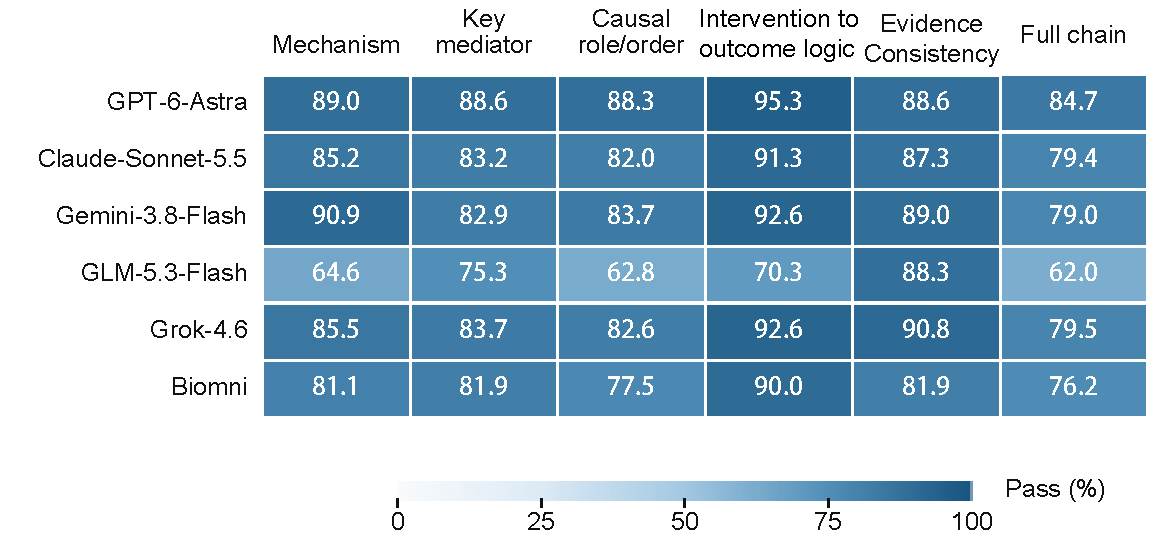
\includegraphics[width=0.7\linewidth]{figs/Fig_4_task2.pdf}
  \captionsetup{skip=2pt}
  \caption{Mechanism-reasoning pass rates of each model in task 2.}
  \label{fig:prompt_task2}
\end{figure}

\subsection{Inverse reasoning performance (Task 3)}



In Task 3, models were given the TF, perturbed entity, target gene and direction of change in target gene expression. They were asked to infer the intervention type and provide a supporting mechanistic reasoning. Task 3's full-chain pass rates, requiring all five mechanistic criteria to be satisfied, ranged from 43.8\% to 72.5\% (Figure~\ref{fig:prompt_task3}). GPT-6-Astra achieved the highest rate (72.5\%), followed by Gemini-3.8-Flash (68.8\%) and Grok-4.6 (66.2\%). Claude-Sonnet-5.5 and GLM-5.3-Flash both achieved 56.2\%, while Biomni had the lowest rate (43.8\%). These full-chain rates assess the reasoning; joint task correctness additionally requires an accepted intervention-type prediction. 

The criterion-level results reveal where the models’ mechanistic reasoning most often fell short. Causal role and order was the lowest-scoring criterion for five of the six models. Performance on causal role was consistently lower than other criteria across most models.  Pass rates for this criterion were particularly low compared with those for intervention-to-outcome logic in Biomni (47.5\% versus 90.0\%) and Gemini-3.8-Flash (71.2\% versus 92.5\%). The PPARA–Pdk4 pair provides a concrete example of an incorrect causal-role assignment. Given BHLHE40 as the perturbed entity and a decrease in Pdk4 expression, models were asked to infer the intervention type. In the curated hepatocyte mechanism, BHLHE40 supports full PPARA-dependent induction, and its depletion by siRNA reduces Pdk4 transcription. A supported explanation must therefore connect the loss of BHLHE40’s coactivating function to reduced PPARA-dependent expression of Pdk4. However, Grok-4.6 explained: \textit{"BHLHE40 functions as a repressive partner transcription factor that antagonizes PPARA at Pdk4 so BHLHE40 overexpression downregulates Pdk4."}. This example also illustrates a limitation of inverse inference. A decrease in target expression alone cannot distinguish depletion of a coactivator from overexpression of a repressor without knowing the relevant regulatory mechanism. These results identify the causal roles and ordering of regulatory components as recurring weaknesses in model-generated explanations, highlighting the importance of assessing intermediate mechanistic steps alongside the relationship between an intervention and the observed response.





\begin{figure}[!htbp]
  \centering
  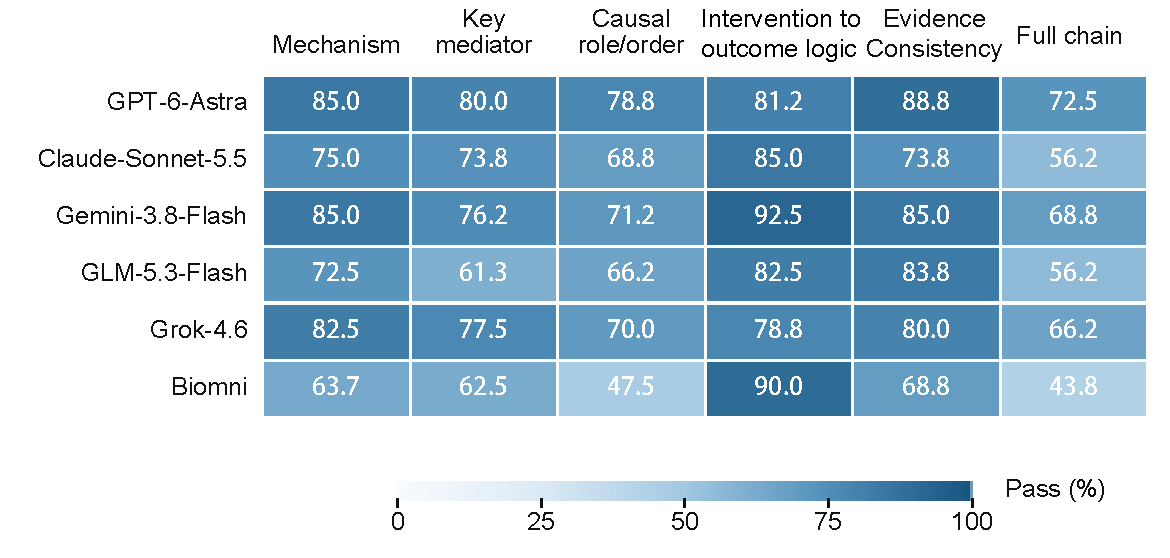
\includegraphics[width=0.7\linewidth]{figs/Fig5_task3.pdf}
  \captionsetup{skip=2pt}
  \caption{Mechanism-reasoning pass rates of each model in task 3.}
  \label{fig:prompt_task3}
\end{figure}

\subsection{Shared failures in mechanistic reasoning across models}

The mechanistic evaluations in Tasks 2 and 3 revealed difficulties in assigning causal roles and ordering regulatory interactions. 
For example, GLM-5.3-Flash achieved the pass rate of 62.8\% for causal role and order in Task 2, while Biomni achieved 47.5\% on the same criterion in Task 3. This criterion requires models to explain whether a component promotes or represses the relevant regulatory process and how its function connects the TF to the target response. The observed errors included both failure to identify necessary regulatory partners and reversal of the functional roles of correctly identified components. 

Several models failed to identify the roles of required regulatory partners. In the curated combinatorial mechanism involving TP63 and FOXK1, Claude-Sonnet-5.5, GLM-5.3-Flash, Grok-4.6 and Biomni omit FOXK1 as a necessary cooperating TF in the seven TF-loss units discussed here. We also found that models misinterpreted regulatory mechanisms by reversing the roles of regulatory components. For example, in the curated chromatin-mediated mechanism, \(\Delta\)Np63\(\alpha\)/SRCAP-dependent H2A.Z deposition represses SAMD9L expression. In their initial (run 1) responses, all six systems treated H2A.Z as supporting TP63-dependent transcriptional activation (Figure~\ref{fig:reasoning_fault}). This inverted interpretation persisted across runs: the five text-only systems reproduced it in all 20 of their unit-runs, while Biomni did so in 3 of its 4 runs. The sole exception was Biomni's run 3, which correctly identified the repressive dependency (TP63 binding $\rightarrow$ SRCAP-mediated repressive H2A.Z deposition $\rightarrow$ blocked RNAPII elongation; H2A.Z loss $\rightarrow$ derepression) and was the only run to pass the full causal-chain evaluation on this unit. Thus, although the explanations appeared biologically plausible and internally coherent, most runs assigned H2A.Z a function that contradicted the experimental evidence. 

These examples identify two distinct weaknesses in the models’ mechanistic reasoning: omission of a required regulatory dependency and inversion of a component’s activating or repressive function. Both affect the connection between a perturbation and the resulting target response. The evaluated systems did not consistently preserve the experimentally supported regulatory dependencies. These examples characterize failures under the supplied inputs and scoring protocol. The appendix provides intervention-specific module analyses, shared-failure denominators and biological interpretation.


%The findings suggest that the evaluated models did not consistently apply the relevant biological functions of TFs and other regulatory components when explaining perturbation effects. They also support evaluating the intermediate mechanistic steps explicitly, because the presence of relevant molecular names and a coherent intervention–response narrative does not establish that the experimentally supported regulatory mechanism has been recovered.




\begin{figure}[!htbp]
  \centering
  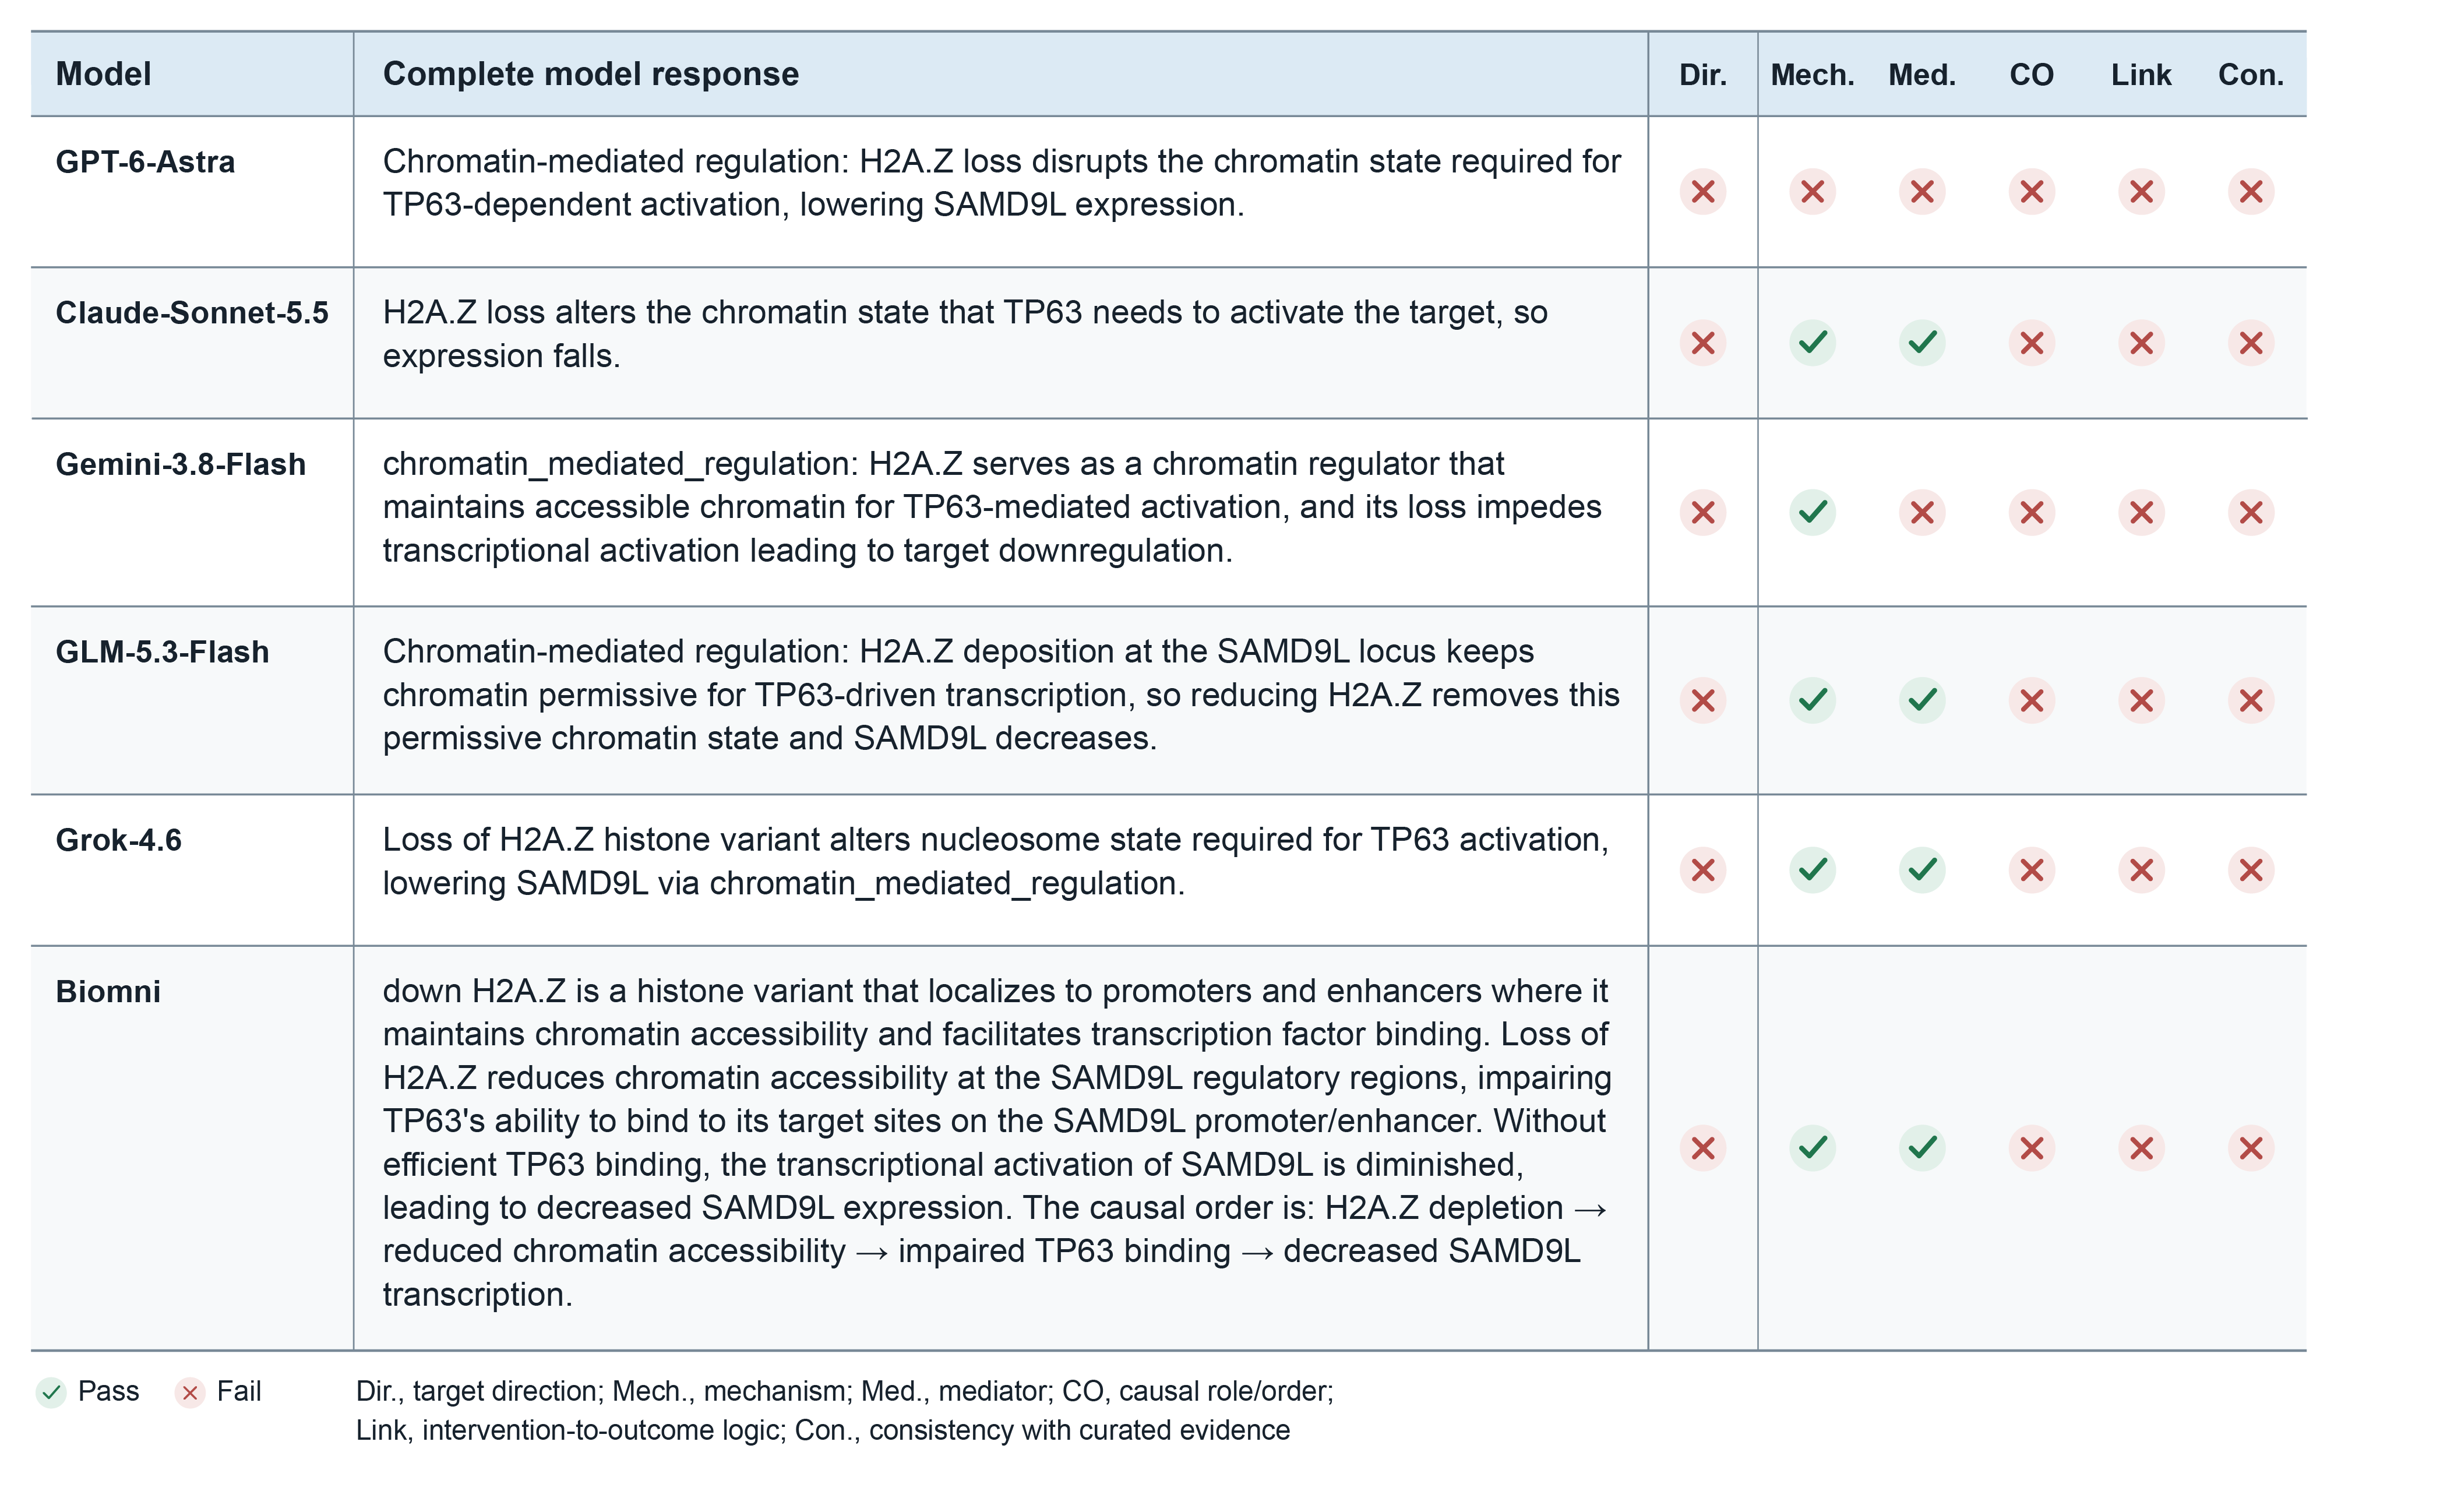
\includegraphics[width=0.8\linewidth]{figs/MeBench_model_response_case-01.png}
  \captionsetup{skip=2pt}
  \caption{Examples of the shared failures in mechanistic reasoning across 6 models.}
  \label{fig:reasoning_fault}
\end{figure}
